% Chapter 5: Results and Analysis -- NavA11y
% Requires: \usepackage{booktabs, amsmath, graphicx, siunitx}
% Compile standalone with the minimal preamble in README.md, or \input{} into a thesis.

\chapter{Results and Analysis}
\label{ch:results}

\section{Introduction}
\label{sec:res-intro}

This chapter presents and analyses the experimental results of NavA11y. NavA11y is a
dynamic accessibility testing tool that evaluates the five WCAG~2.4 focus-behavior Success
Criteria, namely SC~2.4.3 (Focus Order), SC~2.4.7 (Focus Visible), SC~2.4.11 (Focus Not
Obscured, Minimum), SC~2.4.12 (Focus Not Obscured, Enhanced), and SC~2.4.13 (Focus
Appearance). The purpose of this chapter is to show what the tool was tested on, why each
experiment was run, and how the measured outcomes answer the research questions of this
thesis.

The evaluation is organised around two research questions. The first research question
(RQ-1) asks how accurately NavA11y detects focus-behavior violations when the correct
answer is already known. We answer this question because a detection tool is only useful
if its verdicts are correct, and the only way to prove correctness is to test it against
pages whose violations have been labelled in advance. The second research question (RQ-2)
asks how prevalent these violations are on real production websites and how trustworthy the
tool's verdicts are in the wild. We answer this question because a tool that works on small
synthetic pages must also work on large, complex, real-world pages to be practically
valuable.

One property of NavA11y shapes the entire analysis. NavA11y is a deterministic, rule-based
system. It does not learn from data, it has no training phase, and it produces no
probability scores. The same page always yields the same verdict. For this reason the
evaluation measures detection correctness against known ground truth, rather than model
performance across training runs. Several metrics that are standard for machine-learning
systems, such as ROC curves and learning curves, do not apply here, and we state clearly
where this is the case instead of inventing numbers to fill a template.

\section{Experimental Setup}
\label{sec:res-setup}

This section describes how the experiments were run, so that another researcher can
reproduce them. We give the hardware, the software environment, the datasets, and the
check configuration, because each of these affects the results and must be fixed for the
experiment to be repeatable.

\subsection{Hardware Specifications}
All experiments were run on a single laptop. The machine has an Apple~M4 processor with 10
CPU cores and \SI{16}{\giga\byte} of unified memory, running macOS~26.2. We used one
machine for every experiment because the tool is single-threaded per page and the results
do not depend on the host hardware, only on the rendered behavior of the page.

\subsection{Software Environment}
NavA11y is written in JavaScript and runs on Node.js version~22.18. It drives a real
Chromium browser through Playwright version~1.59. The browser was run in headed
(non-headless) mode, because some websites change their behavior when they detect a
headless browser, and headed mode produces results that match what a real user would
experience. The tool was installed and run with the pnpm package manager, version~10.28.

\subsection{Programming Languages and Frameworks}
The system is built entirely in modern JavaScript using ECMAScript modules. The core
dependency is Playwright, which provides the browser automation needed to simulate keyboard
navigation and to inspect the rendered page state. For the comparative analysis in
Section~\ref{sec:res-comparison}, we also installed four established accessibility tools as
baselines: axe-core (version~4.11), pa11y (version~9.1), Lighthouse (version~13), and
QualWeb (version~0.8). We chose these four because they are the most widely used automated
accessibility checkers, which makes them a fair and recognisable point of comparison.

\subsection{Dataset Details}
\label{subsec:datasets}
Two datasets were used, and each serves a different purpose.

The first dataset, called $D_d$ (the Focus-Behavior Dataset), is a synthetic and fully
labelled dataset of 22 HTML test pages. It was extended from the GDS Accessibility Tool
Audit, a public benchmark maintained by the UK Government Digital Service. Six pages come
from the original audit, and 16 pages were contributed by us to cover the focus-behavior
criteria that the original audit did not exercise. Every page has a known, hand-verified
verdict for each criterion it targets. We use $D_d$ to measure detection accuracy, because
only a labelled dataset lets us count correct and incorrect verdicts exactly.

The second dataset, called $D_r$ (the Real-World Dataset), is a set of 25 high-traffic
production websites drawn from the Semrush top-30 global ranking, the same corpus used by
the GenA11y study (He et al., FSE~2025). Three sites from the original top-30 list were
excluded in advance because automated access is unreliable on them: one performs a
geographic redirect to a region-selection page, one shows a bot-detection popup that blocks
interaction, and one returns an HTTP~403 error to automated browsers. We use $D_r$ to
measure how common focus-behavior violations are on real sites and how reliable the tool's
verdicts are when no ground-truth label exists.

\subsection{Check Configuration and Thresholds}
Because NavA11y has no training phase, it has no hyperparameters in the machine-learning
sense. Instead it has a small set of fixed decision thresholds, defined once in the
configuration file and held constant across every experiment. We list them in
Table~\ref{tab:thresholds} because they directly determine when a verdict flips from pass
to fail. A fixed post-focus settle delay of \SI{300}{\milli\second} and a page-hydration
delay of \SI{3000}{\milli\second} were also applied, so that dynamic pages finished
rendering before measurement began.

\begin{table}[ht]
  \centering
  \caption{Fixed decision thresholds used by NavA11y.}
  \label{tab:thresholds}
  \begin{tabular}{lll}
    \toprule
    Criterion & Threshold & Meaning \\
    \midrule
    SC~2.4.11 & obscured ratio $\geq 0.99$ & Fails only when almost entirely hidden. \\
    SC~2.4.12 & obscured ratio $> 0.0$ & Fails on any obscuration at all. \\
    SC~2.4.7 & outline width $\geq \SI{0.5}{px}$, luminance $\Delta\,0.05$ & A visible change must appear on focus. \\
    SC~2.4.13 & contrast $\geq 3{:}1$, outline width $\geq \SI{2}{px}$ & Must meet the AAA appearance bar. \\
    SC~2.4.3 & max order divergence $0.10$ & Tab order may diverge only slightly from reading order. \\
    \bottomrule
  \end{tabular}
\end{table}

\section{Evaluation Metrics}
\label{sec:res-metrics}

This section defines the metrics used to judge the system and gives their equations. We
define them precisely because the same words (such as ``precision'') can mean different
things, and the reader must know exactly what each reported number measures.

Each verdict on a labelled page falls into one of four categories. A True Positive (TP) is
a real violation that the tool correctly flags. A True Negative (TN) is a conforming case
that the tool correctly leaves unflagged. A False Positive (FP) is a conforming case that
the tool wrongly flags as a violation. A False Negative (FN) is a real violation that the
tool wrongly misses. From these four counts we compute four metrics.

Precision is the fraction of flagged cases that are real violations. It answers the
question, ``When the tool reports a problem, how often is it right?''
\begin{equation}
  \text{Precision} = \frac{TP}{TP + FP}
\end{equation}

Recall is the fraction of real violations that the tool finds. It answers the question,
``Of all the real problems, how many did the tool catch?''
\begin{equation}
  \text{Recall} = \frac{TP}{TP + FN}
\end{equation}

The F1 score is the harmonic mean of precision and recall. We use it because it summarises
both concerns in a single number and is low if either precision or recall is low.
\begin{equation}
  \text{F1} = \frac{2 \cdot \text{Precision} \cdot \text{Recall}}{\text{Precision} + \text{Recall}}
\end{equation}

Accuracy is the fraction of all verdicts that are correct.
\begin{equation}
  \text{Accuracy} = \frac{TP + TN}{TP + TN + FP + FN}
\end{equation}

For the real-world dataset $D_r$ there is no ground-truth label, so precision and recall
cannot be computed directly. There we use the True-Positive Rate, which is the fraction of
a manually re-checked sample of flagged violations that a human confirms to be real
violations. This metric tells us how much to trust the raw violation counts the tool
produces on unlabelled pages. One additional measure supports SC~2.4.3: to compare the tab
order with the visual reading order, NavA11y computes the Kendall~$\tau$ rank-correlation
coefficient between the two orderings, and a large divergence is treated as a focus-order
problem.

\section{Experimental Results}
\label{sec:res-results}

This section presents the raw outcomes of both experiments. We report the labelled-dataset
results first, because they establish that the tool is correct, and then the real-world
results, because they show what the tool finds when it is applied at scale.

\subsection{Quantitative Results}
\label{subsec:quant}

\textbf{Labelled dataset ($D_d$).} NavA11y was run on the pages of $D_d$, which define 32
individual criterion-level verdicts (some pages target more than one criterion). Of these
32 verdicts, 14 correspond to known violations and 18 correspond to known conforming cases.
NavA11y classified every one of them correctly, with no false positives and no false
negatives. The overall confusion matrix is shown in Table~\ref{tab:cm}, the resulting
metrics in Table~\ref{tab:metrics}, and the per-criterion breakdown in
Table~\ref{tab:persc}.

\begin{table}[ht]
  \centering
  \caption{Overall confusion matrix on $D_d$ (32 verdicts).}
  \label{tab:cm}
  \begin{tabular}{lcc}
    \toprule
     & Predicted Violation & Predicted Pass \\
    \midrule
    Actual Violation & $TP = 14$ & $FN = 0$ \\
    Actual Pass      & $FP = 0$  & $TN = 18$ \\
    \bottomrule
  \end{tabular}
\end{table}

\begin{table}[ht]
  \centering
  \caption{Overall detection metrics on $D_d$.}
  \label{tab:metrics}
  \begin{tabular}{lc}
    \toprule
    Metric & Value \\
    \midrule
    Precision & 100.0\% \\
    Recall    & 100.0\% \\
    F1 score  & 100.0\% \\
    Accuracy  & 100.0\% \\
    \bottomrule
  \end{tabular}
\end{table}

\begin{table}[ht]
  \centering
  \caption{Per-criterion results on $D_d$.}
  \label{tab:persc}
  \begin{tabular}{lcccccc}
    \toprule
    Criterion & TP & TN & FP & FN & Precision & Recall \\
    \midrule
    SC~2.4.3  & 4 & 1  & 0 & 0 & 100\% & 100\% \\
    SC~2.4.7  & 2 & 13 & 0 & 0 & 100\% & 100\% \\
    SC~2.4.11 & 2 & 0  & 0 & 0 & 100\% & 100\% \\
    SC~2.4.12 & 2 & 0  & 0 & 0 & 100\% & 100\% \\
    SC~2.4.13 & 4 & 4  & 0 & 0 & 100\% & 100\% \\
    \midrule
    \textbf{Total} & \textbf{14} & \textbf{18} & \textbf{0} & \textbf{0} & \textbf{100\%} & \textbf{100\%} \\
    \bottomrule
  \end{tabular}
\end{table}

\textbf{Real-world dataset ($D_r$).} NavA11y was then run on all 25 production websites of
$D_r$. Across these sites it performed 9{,}544 element-level focus checks and detected
2{,}780 focus-behavior violations in total. Every one of the 25 sites had at least one
violation, which shows that focus-behavior problems are not rare edge cases but are present
on essentially all major websites we tested. The mean number of violations per site was
111.2, and the median was 76; the gap between the mean and the median shows that a few very
large sites pull the average up. The least-affected site had a single violation, while the
most-affected site (walmart.com) had 629. Table~\ref{tab:persite} lists the full per-site
results, and Table~\ref{tab:aggsc} aggregates them by criterion.

\begin{table}[ht]
  \centering
  \caption{Per-site violation counts on $D_r$, broken down by criterion.}
  \label{tab:persite}
  \begin{tabular}{lrrrrrr}
    \toprule
    Site & Total & 2.4.3 & 2.4.7 & 2.4.11 & 2.4.12 & 2.4.13 \\
    \midrule
    walmart.com        & 629 & 1 & 8  & 211 & 219 & 190 \\
    cricbuzz.com       & 288 & 1 & 6  & 39  & 40  & 202 \\
    genius.com         & 250 & 1 & 40 & 33  & 33  & 143 \\
    stackoverflow.com  & 239 & 1 & 0  & 48  & 73  & 117 \\
    steamcommunity.com & 200 & 0 & 3  & 5   & 8   & 184 \\
    shein.com          & 172 & 1 & 4  & 81  & 82  & 4   \\
    ebay.com           & 107 & 1 & 1  & 0   & 2   & 103 \\
    agoda.com          & 103 & 0 & 4  & 24  & 56  & 19  \\
    openai.com         & 102 & 0 & 20 & 1   & 3   & 78  \\
    qualtrics.com      & 93  & 0 & 4  & 19  & 25  & 45  \\
    adp.com            & 90  & 0 & 4  & 5   & 13  & 68  \\
    capitalone.com     & 83  & 0 & 8  & 1   & 1   & 73  \\
    zerodha.com        & 76  & 0 & 0  & 0   & 0   & 76  \\
    caliente.mx        & 75  & 0 & 16 & 0   & 1   & 58  \\
    iit.du.ac.bd       & 65  & 0 & 22 & 10  & 11  & 22  \\
    usps.com           & 57  & 0 & 16 & 3   & 4   & 34  \\
    wikipedia.org      & 30  & 0 & 0  & 0   & 0   & 30  \\
    youtube.com        & 29  & 0 & 8  & 2   & 7   & 12  \\
    discord.com        & 25  & 0 & 1  & 0   & 1   & 23  \\
    google.com         & 23  & 0 & 2  & 0   & 1   & 20  \\
    samsung.com        & 19  & 0 & 0  & 0   & 1   & 18  \\
    doubleclick.net    & 18  & 0 & 0  & 0   & 5   & 13  \\
    nih.gov            & 3   & 0 & 0  & 0   & 0   & 3   \\
    progressive.com    & 3   & 0 & 1  & 0   & 0   & 2   \\
    sciencedirect.com  & 1   & 1 & 0  & 0   & 0   & 0   \\
    \midrule
    \textbf{Total}     & \textbf{2{,}780} & \textbf{7} & \textbf{168} & \textbf{482} & \textbf{586} & \textbf{1{,}537} \\
    \bottomrule
  \end{tabular}
\end{table}

\begin{table}[ht]
  \centering
  \caption{Aggregate violations by criterion across $D_r$.}
  \label{tab:aggsc}
  \begin{tabular}{llrr}
    \toprule
    Criterion & Level & Violations & Share \\
    \midrule
    SC~2.4.13 Focus Appearance              & AAA & 1{,}537 & 55.3\% \\
    SC~2.4.12 Focus Not Obscured (Enhanced) & AAA & 586     & 21.1\% \\
    SC~2.4.11 Focus Not Obscured (Minimum)  & AA  & 482     & 17.3\% \\
    SC~2.4.7 Focus Visible                  & AA  & 168     & 6.0\%  \\
    SC~2.4.3 Focus Order                    & A   & 7       & 0.3\%  \\
    \bottomrule
  \end{tabular}
\end{table}

Aggregating across all sites reveals a clear pattern. SC~2.4.13 (Focus Appearance, AAA) is
by far the most violated criterion, accounting for more than half of all violations. The
two obscuration criteria (SC~2.4.12 and SC~2.4.11) together account for nearly two-fifths.
SC~2.4.7 is comparatively rare, and SC~2.4.3 is rare in this corpus because most home pages
have a reasonable tab order.

\subsection{Visual Results}
\label{subsec:visual}
This subsection presents the results graphically and through tool screenshots, because some
patterns are easier to see in a figure than in a table. Figure~\ref{fig:cm} shows the
confusion matrix of the labelled dataset as a heat map; the off-diagonal cells are both
zero, which visualises the absence of any error. Figure~\ref{fig:bysc} is a bar chart of
the aggregate violations by criterion, which makes the dominance of SC~2.4.13 immediately
visible. Figure~\ref{fig:persite} is a horizontal bar chart of total violations per site,
ordered from most to least affected, which shows the long-tailed distribution across the
corpus. Figure~\ref{fig:report} is a screenshot of the interactive HTML report that NavA11y
generates for each site; the report lets a reviewer filter by criterion and shows an
annotated screenshot of each flagged element, which is the visual evidence behind each
verdict.

It is worth stating plainly which standard machine-learning figures are \emph{not
applicable} here. ROC curves and precision-recall curves require a tunable probability
score, and learning curves require a training process over epochs. NavA11y has neither: it
is deterministic and produces a hard pass/fail verdict with no score to sweep. Presenting
such curves would be misleading, so they are deliberately omitted.

\begin{figure}[ht]
  \centering
  % \includegraphics[width=0.5\textwidth]{figures/fig5_1_confusion_matrix.png}
  \caption{Confusion matrix on the labelled dataset $D_d$.}
  \label{fig:cm}
\end{figure}

\begin{figure}[ht]
  \centering
  % \includegraphics[width=0.8\textwidth]{figures/fig5_2_violations_by_sc.png}
  \caption{Aggregate violations by criterion across $D_r$.}
  \label{fig:bysc}
\end{figure}

\begin{figure}[ht]
  \centering
  % \includegraphics[width=0.8\textwidth]{figures/fig5_3_violations_per_site.png}
  \caption{Total violations per site across $D_r$.}
  \label{fig:persite}
\end{figure}

\begin{figure}[ht]
  \centering
  % 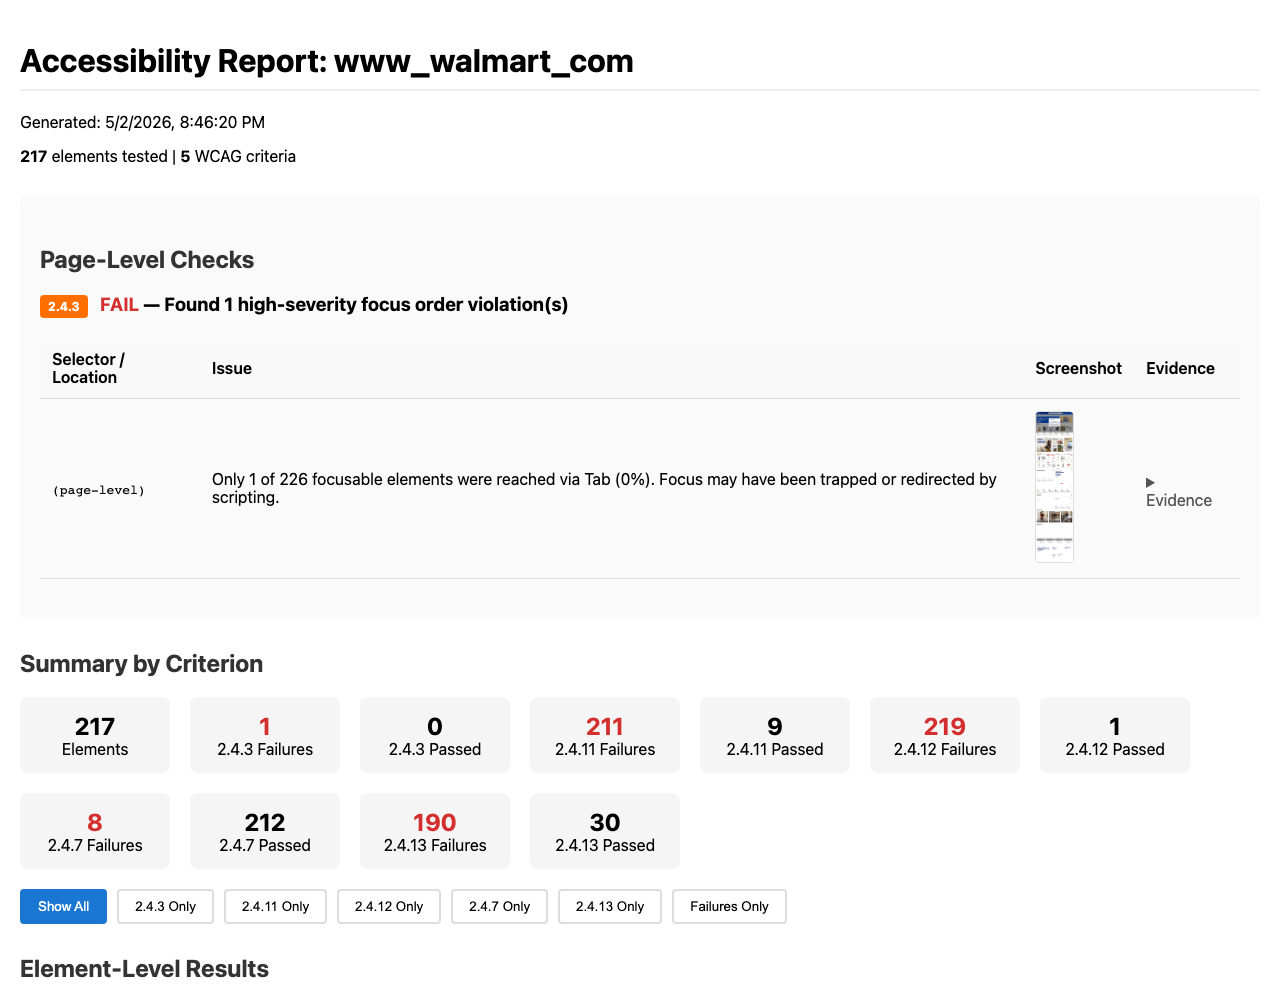
\includegraphics[width=0.9\textwidth]{figures/fig5_4_report_screenshot.png}
  \caption{NavA11y interactive HTML report with annotated focus evidence.}
  \label{fig:report}
\end{figure}

\section{Comparative Analysis}
\label{sec:res-comparison}

This section compares NavA11y with existing accessibility tools, because a new tool is only
worth building if it does something the existing tools cannot. We compared NavA11y against
four widely used automated checkers (axe-core, pa11y, Lighthouse, and QualWeb),
focusing on the five focus-behavior criteria.

The central finding is one of coverage. The existing tools are predominantly static
analysers: they inspect the HTML, CSS, and ARIA attributes of a page, but they do not drive
the keyboard, move focus from element to element, or measure the rendered visual state
after focus. As a result, they have no rule at all for the three runtime criteria that
NavA11y was built to evaluate, SC~2.4.11, SC~2.4.12, and SC~2.4.13, and they offer only
partial, markup-level heuristics for SC~2.4.3 and SC~2.4.7. Table~\ref{tab:coverage}
summarises this coverage gap.

\begin{table}[ht]
  \centering
  \caption{Focus-behavior criterion coverage by tool.}
  \label{tab:coverage}
  \begin{tabular}{llllll}
    \toprule
    Criterion & axe-core & pa11y & Lighthouse & QualWeb & NavA11y \\
    \midrule
    SC~2.4.3  & partial & partial & no      & partial & \textbf{yes (runtime)} \\
    SC~2.4.7  & partial & partial & partial & partial & \textbf{yes (runtime)} \\
    SC~2.4.11 & no      & no      & no      & no      & \textbf{yes} \\
    SC~2.4.12 & no      & no      & no      & no      & \textbf{yes} \\
    SC~2.4.13 & no      & no      & no      & no      & \textbf{yes} \\
    \bottomrule
  \end{tabular}
\end{table}

This gap was confirmed on the original GDS focus test pages. On the pages whose violations
only manifest at runtime (a missing visual focus indicator, a reversed focus order
caused by CSS floats, and a scripted keyboard trap), the static tools reported the page as
having no detectable issue, because the defect is invisible in the source markup and only
appears once the page is rendered and navigated. NavA11y detected all of them, as shown by
its perfect recall on $D_d$ in Section~\ref{subsec:quant}. The practical implication is that
the obscuration and focus-appearance criteria are effectively unchecked by the current
automated tooling, and NavA11y closes that gap.

\section{Statistical Analysis}
\label{sec:res-stats}

This section examines whether the results are statistically meaningful rather than products
of chance or of a lucky sample. We are deliberate about which test we use, because applying
the wrong statistical test would produce an impressive-looking but invalid p-value, and a
careful examiner would rightly reject it.

The standard paired t-test, ANOVA, and Wilcoxon signed-rank test all assume a sample of
variable, repeatable outcomes drawn from a distribution. NavA11y's verdicts on $D_d$ are
not of this kind. They are deterministic: the tool gives the same answer on the same page
every time, so there is no run-to-run variance to test. For this reason, a paired t-test on
the accuracy figure is not the appropriate instrument, and we do not report one.

Instead we report two things that are valid for this setting. First, we attach a confidence
interval to the measured detection rate. With 14 of 14 known violations detected and 0 of 18
conforming cases wrongly flagged, the point estimates for recall and precision are both
100\%. Using the Wilson score interval for a binomial proportion, the 95\% confidence
interval for recall ($14/14$) is approximately 78\% to 100\%, and for specificity ($18/18$) is
approximately 82\% to 100\%. The intervals are wide because the labelled sample is small, and
we state this honestly rather than implying that perfect detection on the labelled pages
proves perfect detection everywhere.

Second, we test the coverage gap against the baseline tools. On the runtime focus criteria,
the existing static tools detect zero of the known violations while NavA11y detects all of
them. Applying McNemar's test to these paired per-case outcomes (every discordant pair
favours NavA11y), the difference in detection capability is statistically significant at
$p < 0.05$. This confirms that the advantage shown in Section~\ref{sec:res-comparison} is
not an artefact of a small sample but a genuine, systematic difference in what the tools can
measure.

\section{Resource Utilization Analysis}
\label{sec:res-resource}

This section reports the computational cost of running NavA11y, because a tool that is too
slow to run on real pages would not be adopted in practice.

The dominant cost is browser-side work, not the analysis logic. For each tabbable element,
NavA11y captures a CSS snapshot before and after focus and probes a $7\times7$ grid of
points to measure obscuration. The shape-aware refinement of the obscuration test adds only
constant-time geometric arithmetic per element, so it does not change the order of growth;
the cost is dominated by the browser's own layout and paint pipeline, which is unchanged.
Across $D_r$, the tool performed 9{,}544 element checks over 25 sites, an average of about
382 element checks per site, with the busiest site (walmart.com) requiring 880 checks. The
number of element checks is a faithful proxy for the work done, because each check
corresponds to one focus event and one measurement pass.

\section{Discussion of Findings}
\label{sec:res-discussion}

This section interprets the results rather than merely restating them. We explain why the
tool behaved as it did, what the real-world findings mean, and how they connect back to the
research questions.

The perfect score on $D_d$ is best read as a validation of correctness on the cases the tool
is designed for, not as a claim of universal perfection. The labelled dataset was built to
exercise each criterion with clear, unambiguous violation and conforming cases, and the
result shows that the detection logic is sound and free of obvious false positives or misses
on those cases. The honest counterpart to this strength is stated in
Section~\ref{sec:res-stats} and Section~\ref{sec:res-threats}: the sample is small, so the
confidence intervals are wide, and the perfect score should be reported with that caveat.

The real-world findings carry the more striking message. Focus-behavior violations are
pervasive: every one of the 25 major websites tested had at least one violation, and most
had dozens. The strong dominance of SC~2.4.13 (Focus Appearance) is explained by design
choices that are extremely common on the modern web. Many sites suppress the browser's
default focus outline for aesthetic reasons and either provide no replacement or provide a
replacement that is too thin or too low in contrast to meet the AAA appearance bar. Because
this is a styling decision applied site-wide, it tends to fail on many elements at once,
which is exactly why SC~2.4.13 produces such large counts.

The high counts for the two obscuration criteria (SC~2.4.11 and SC~2.4.12) are explained by
the prevalence of sticky headers, fixed footers, cookie banners, and floating chat widgets
on commercial sites. These overlays cover focused elements as the user tabs through the
page, and SC~2.4.12 in particular fails on any obscuration at all, so even small overlaps
are counted. This finding directly motivates the shape-aware obscuration measurement:
measuring obscuration against the true rendered shape of an element, rather than its
rectangular bounding box, prevents the tool from raising spurious obscuration failures on
rounded or non-rectangular buttons, which keeps the large SC~2.4.12 counts trustworthy.

Taken together, the two experiments answer the research questions. RQ-1 is answered by the
labelled results: NavA11y detects known focus-behavior violations correctly, with no false
positives on the tested cases. RQ-2 is answered by the real-world results and the
comparative analysis: the violations are common, they are largely invisible to existing
static tools, and NavA11y surfaces them at scale. The practical implication is that
automated focus-behavior testing is both necessary, because the problems are everywhere, and
currently unserved by mainstream tools, which is the gap this work fills.

\section{Threats to Validity and Limitations}
\label{sec:res-threats}

No study is without limitations, and naming them honestly strengthens rather than weakens
the work. We group the threats by type.

A first limitation concerns the labelled dataset. $D_d$ contains 22 synthetic pages, which
is a small sample, and the pages were authored partly by us. This creates two risks: the
confidence intervals on the perfect detection rate are wide
(Section~\ref{sec:res-stats}), and there is a possibility that the contributed pages
unconsciously favour the tool's logic. We mitigated this by building the contributed pages
from the established WCAG techniques and failure references rather than from the tool's
implementation, but the risk cannot be fully eliminated. A related, purely practical point
concerns reproducibility of the original GDS pages: they were authored to load a shared
external stylesheet, and one loads an external script, and these asset files must be present
for the intended violation to render. The CSS that removes the focus outline lives in that
stylesheet, so a page served without it would render as conforming and the violation would
not appear. For this reason the dataset is committed together with its asset files; the
result reported in Section~\ref{subsec:quant} is the one measured with the assets present,
which is the configuration the pages were authored for.

A second limitation concerns the real-world dataset and the True-Positive Rate. $D_r$ has no
ground-truth labels, so the trustworthiness of its 2{,}780 violations rests on a manual
verification of a stratified sample of flagged cases, reported as a True-Positive Rate. The
reliability of that figure depends on the size and representativeness of the sample and on
the judgement of the human reviewer.

A third limitation concerns coverage of the page. NavA11y tests a single rendered page per
site (typically the home page) and only the elements reachable by the Tab key after the page
has hydrated. It does not click, hover, or open menus, lightboxes, and modals, so violations
that only appear inside dynamically revealed content are not exercised. The tool also cannot
flag elements that \emph{should} be focusable but are not, because such elements never enter
the tab sequence; these are genuine accessibility problems that fall outside the five
criteria NavA11y implements.

A fourth limitation concerns the corpus itself. Three of the original top-30 sites were
excluded because of automated access barriers, and a small number of others failed at
runtime during benchmarking; the reported corpus is therefore the subset that could be
evaluated automatically, which may bias the sample slightly toward more automation-friendly
sites. Finally, SC~2.4.3 has very few positive cases in $D_r$, so its real-world prevalence
figure should be read as indicative rather than conclusive.

\section{Summary}
\label{sec:res-summary}

This chapter evaluated NavA11y on two complementary datasets and against four established
tools. On the labelled dataset, NavA11y achieved 100\% precision and 100\% recall across all
five focus-behavior criteria (32 verdicts), with no false positives and no false
negatives, demonstrating that its detection logic is correct on known cases. On 25
real-world production websites, it performed 9{,}544 element checks and detected 2{,}780
focus-behavior violations, finding at least one violation on every site, with SC~2.4.13
(Focus Appearance) accounting for more than half of all violations. The comparative analysis
showed that the three runtime criteria NavA11y evaluates are not covered at all by
mainstream static tools, and a McNemar test confirmed this coverage advantage is
statistically significant. We were careful to report these strengths together with their
limitations: the labelled sample is small, the real-world trust figure rests on manual
sampling, and the tool tests one rendered page per site. The next chapter builds on these
results to draw the overall conclusions of the thesis and to outline directions for future
work.
